\newpage
\begin{flushleft}
{\fontsize{16pt}{16pt}\selectfont \textbf{CHAPTER 5}}
\end{flushleft}		
\begin{center}
{\fontsize{18pt}{22pt}\selectfont \textbf{PROJECT DESCRIPTION}}\\[2mm]
\end{center}
\addcontentsline{toc}{section}{\numberline{5}PROJECT DESCRIPTION}

\onehalfspacing
\justifying
\noindent This chapter provides an exhaustive architectural and structural decomposition of SmartCampus AI. It details the high-level system architecture, describes the individual operational modules, and formalizes system dynamics through Data Flow Diagrams (DFDs), Unified Modeling Language (UML) Use Case models, and Sequence Diagrams.

\vspace{0.2in}
\begin{flushleft}
{\fontsize{14pt}{18pt}\selectfont \textbf{5.1 PROBLEM DEFINITION}}\\[2mm]
\end{flushleft}
\addcontentsline{toc}{subsection}{\numberline{5.1}Problem Definition}

\noindent Higher education institutions require an automated, tamper-proof, and real-time mechanism to track student attendance and analyze classroom engagement without wasting valuable instructional time. Traditional paper registers, door-mounted card readers, and manual roll calls are slow, susceptible to proxy marking, and provide zero visibility into in-class learning dynamics. SmartCampus AI addresses this challenge by ingesting overhead classroom CCTV video, detecting and recognizing student identities using deep metric learning, clustering un-enrolled students automatically, enforcing mathematical conflict prevention, and generating real-time behavioral telemetry.

\vspace{0.2in}
\begin{flushleft}
{\fontsize{14pt}{18pt}\selectfont \textbf{5.2 OVERVIEW OF THE PROJECT}}\\[2mm]
\end{flushleft}
\addcontentsline{toc}{subsection}{\numberline{5.2}Overview of the Project}

\noindent SmartCampus AI is an enterprise-grade biometric identity lifecycle and classroom engagement analytics platform. The system operates autonomously over multi-camera classroom RTSP feeds, executing an end-to-end computer vision pipeline comprising SCRFD-10G face detection, Laplacian blur filtering, 5-point landmark affine normalization, 512D ArcFace embeddings, and sub-millisecond FAISS vector indexing. An unsupervised density-based clustering engine (HDBSCAN) discovers student identities from video tracks, presenting representative crops to teachers in a zero-refresh verification portal. An automated Conflict Prevention Engine enforces bijective identity mappings. In parallel, real-time posture analysis evaluates student alertness, flags fatigue or phone distractions, and routes instant WebSocket alerts to educators.

\vspace{0.2in}
\begin{flushleft}
{\fontsize{14pt}{18pt}\selectfont \textbf{5.3 SYSTEM ARCHITECTURE}}\\[2mm]
\end{flushleft}
\addcontentsline{toc}{subsection}{\numberline{5.3}System Architecture}

\noindent Figure 5.1 illustrates the high-level distributed microservice architecture of SmartCampus AI, organized across Edge Sensing, AI Vision Engine, Vector Repository, API Gateway, and Web Client layers.

\begin{figure}[h]
    \centering
    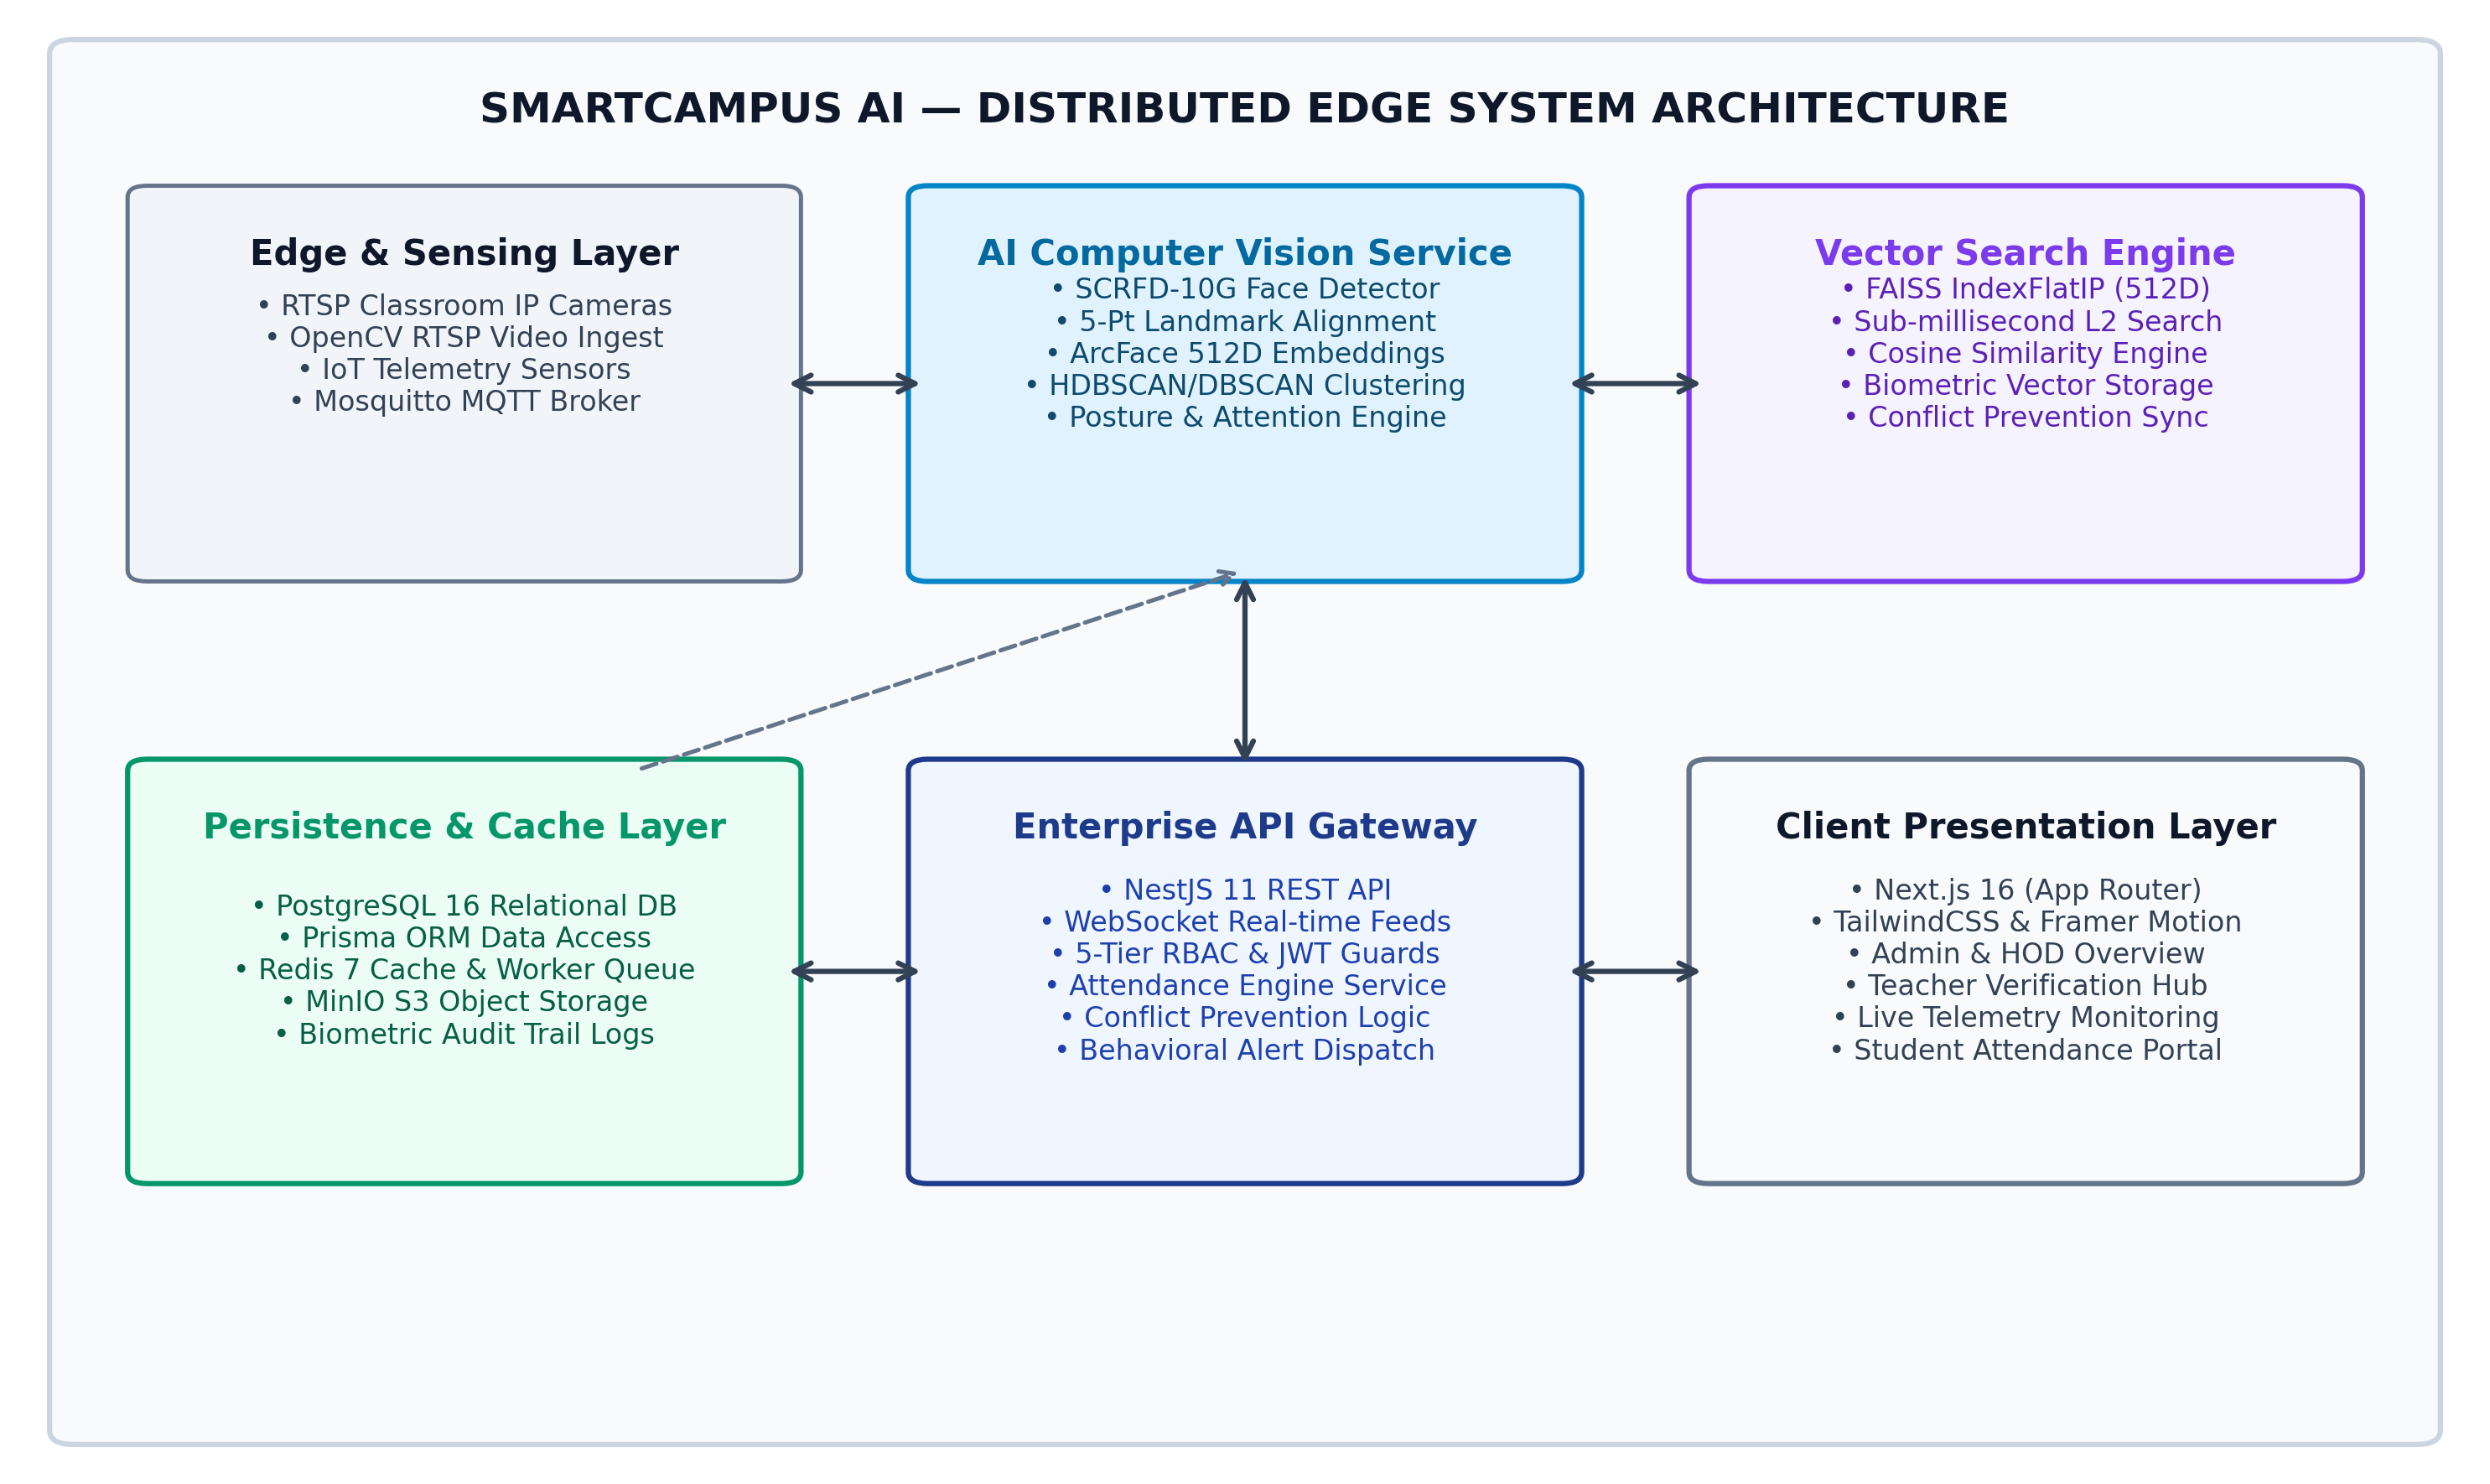
\includegraphics[width=0.92\textwidth]{assets/fig_architecture.png}
    \caption{System Architecture of the SmartCampus AI Platform}
    \label{fig:sys_arch}
\end{figure}

\vspace{0.2in}
\begin{flushleft}
{\fontsize{14pt}{18pt}\selectfont \textbf{5.4 MODULE DESCRIPTION}}\\[2mm]
\end{flushleft}
\addcontentsline{toc}{subsection}{\numberline{5.4}Module Description}

\noindent The system is organized into eight specialized, decoupled functional modules:
\begin{enumerate}
    \item \textbf{Module 1: Edge Sensing \& Video Ingestion Module:} Connects to classroom IP cameras via RTSP, decodes H.264 video streams at 25 FPS, buffers raw RGB frames in memory queues, and provides a synthetic `MockVideoCapture` fallback for headless development.
    \item \textbf{Module 2: AI Face Detection, Alignment \& Blur Filtering:} Applies SCRFD-10G to extract face bounding boxes and 5 landmarks, evaluates Laplacian variance blur metric $\sigma^2_\Delta \ge 120.0$, and executes affine transformation to normalize crops to $112 \times 112$ px.
    \item \textbf{Module 3: Deep Metric Feature Extraction \& FAISS Vector Matching:} Processes aligned crops through ResNet-100 ArcFace deep neural networks, produces 512-dimensional L2-normalized feature embeddings, and executes cosine similarity matching in an in-memory FAISS `IndexFlatIP` repository with threshold $\tau = 0.65$.
    \item \textbf{Module 4: Unsupervised Identity Candidate Clustering:} In unassigned sessions, groups recurring face appearances across temporal tracks using HDBSCAN/DBSCAN into distinct candidate clusters, computing composite quality scores $Q(I)$ to extract the sharpest frontal crop.
    \item \textbf{Module 5: Conflict Prevention \& Bidirectional Sync Engine:} Mathematically guarantees bijective identity mappings ($\text{Card}(S \cap C) \le 1$). When a teacher verifies a student for a cluster, any conflicting prior assignment is automatically released, and confirmed vectors are synced into FAISS and PostgreSQL.
    \item \textbf{Module 6: In-Class Behavioral Analytics \& Attention Index Scoring:} Monitors student head pitch, yaw, and eye aspect ratios, calculating an Attention Index score (0\% to 100\%) and classifying states into Alert ($\ge 80\%$), Drowsy ($< 40\%$), and Smartphone Distracted.
    \item \textbf{Module 7: Headcount Normalization \& Role-Based Alert Dispatcher:} Segregates active in-class attendees (18 seated in Room 408) from broader batch rosters (59 enrolled students), bounds unknown visitor counters, and dispatches real-time WebSocket alert toasts to instructors and HODs.
    \item \textbf{Module 8: Full-Stack Web Portal \& Administrative Analytics:} Next.js 16 glassmorphism client portal and NestJS 11 gateway providing responsive dashboards for Super Admins, College Admins, Dept HODs, Teachers, and Students.
\end{enumerate}

\vspace{0.2in}
\begin{flushleft}
{\fontsize{14pt}{18pt}\selectfont \textbf{5.5 DATA FLOW DIAGRAM}}\\[2mm]
\end{flushleft}
\addcontentsline{toc}{subsection}{\numberline{5.5}Data Flow Diagram}

\noindent Figure 5.2 depicts the Data Flow Diagram (DFD Level 0 Context Diagram) illustrating the flow of RTSP frames, session activation commands, attendance ledgers, and WebSocket alerts.

\begin{figure}[h]
    \centering
    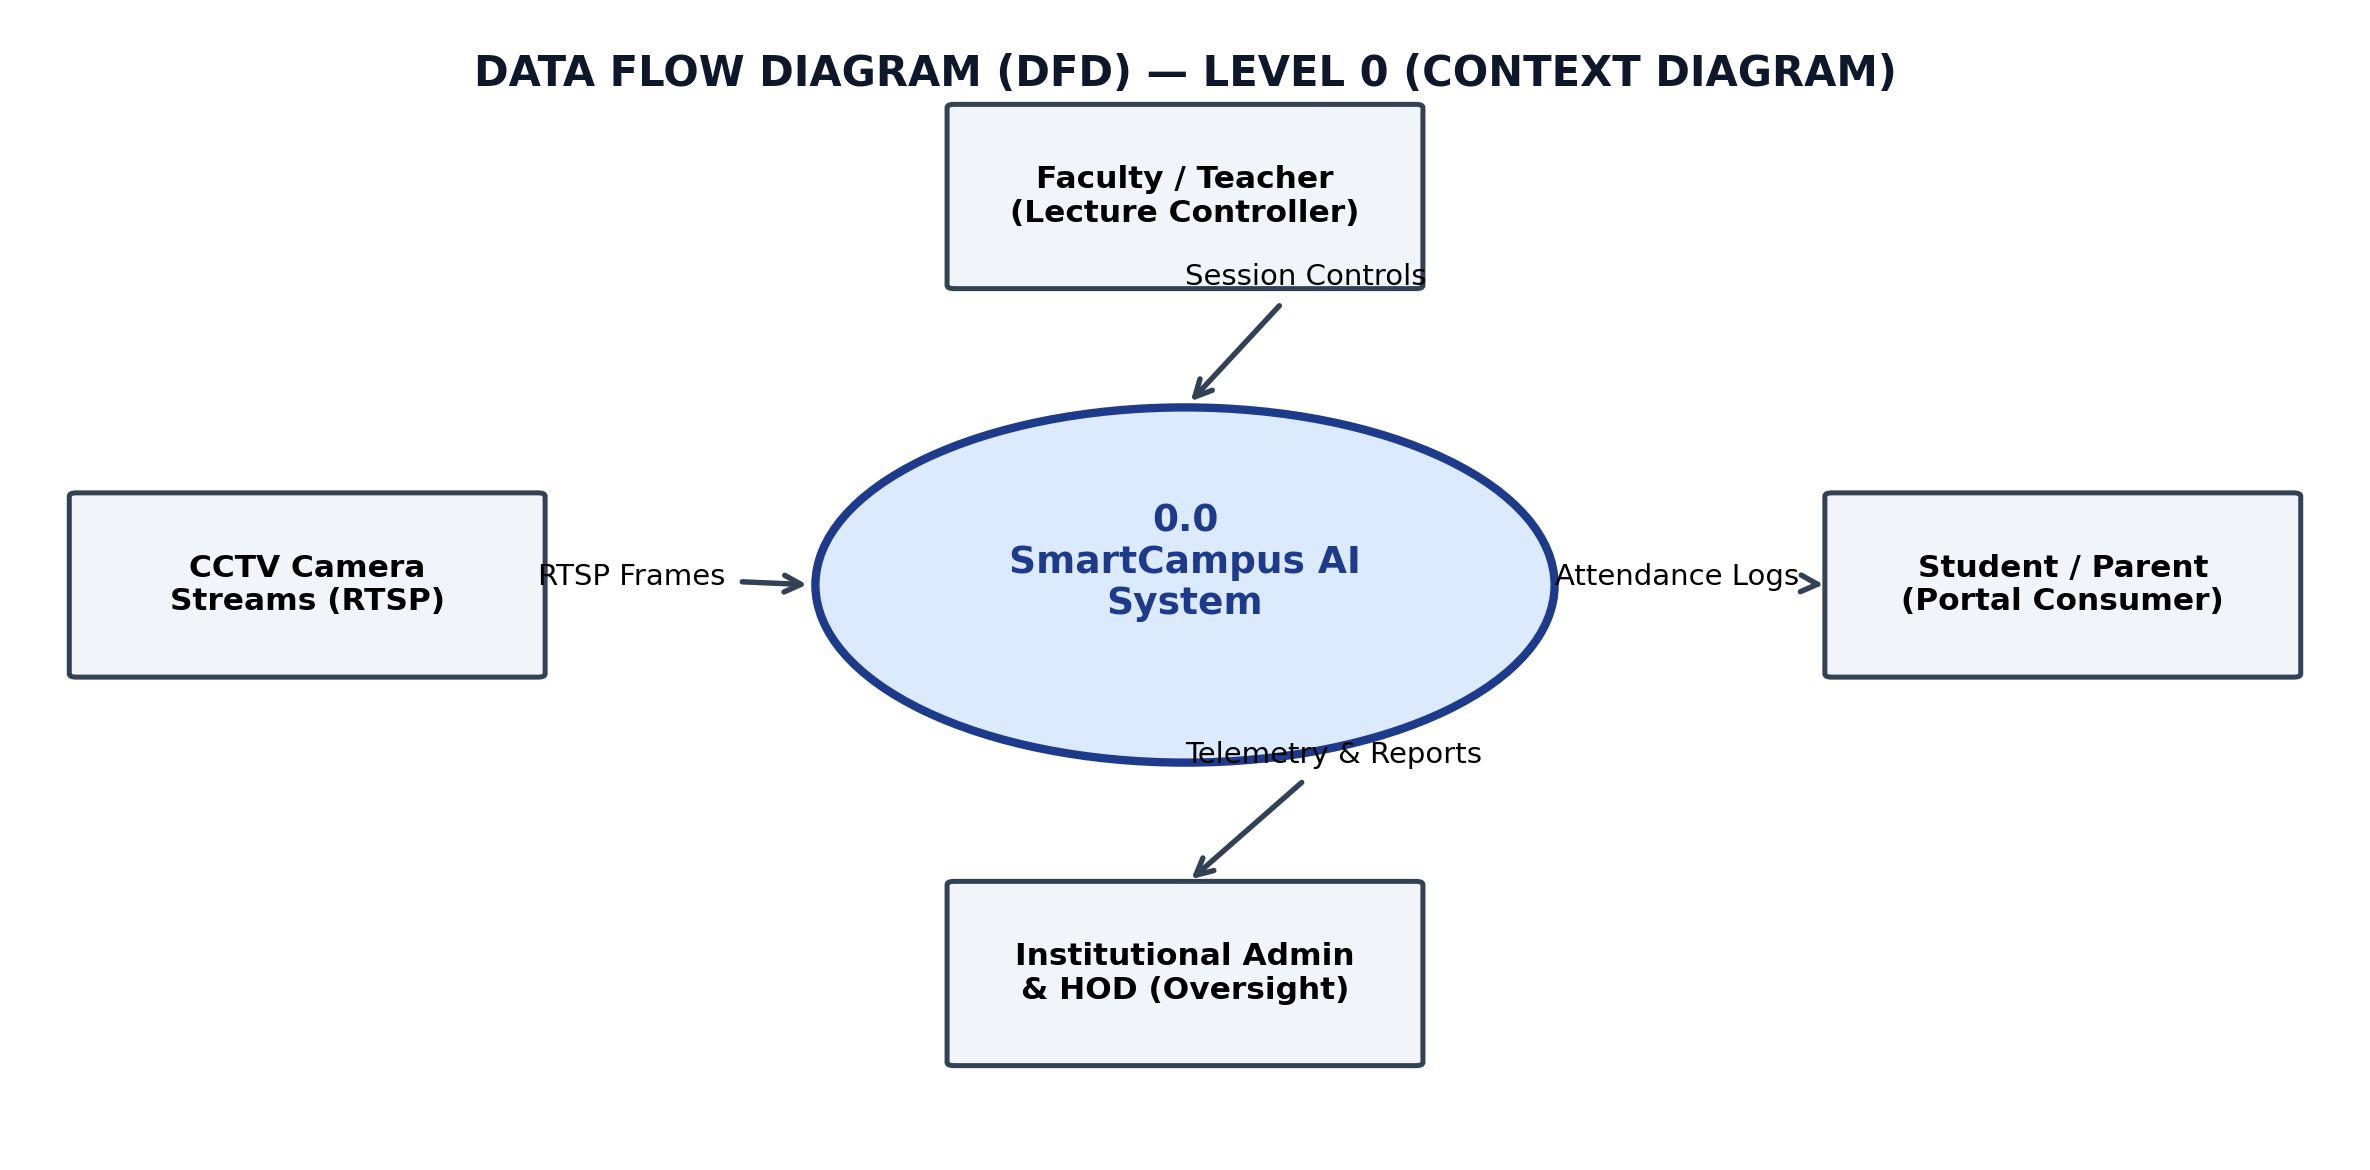
\includegraphics[width=0.85\textwidth]{assets/fig_dfd_lvl0.png}
    \caption{Data Flow of SmartCampus AI (Level 0 Context Diagram)}
    \label{fig:dfd}
\end{figure}

\vspace{0.2in}
\begin{flushleft}
{\fontsize{14pt}{18pt}\selectfont \textbf{5.6 USE CASE DIAGRAM}}\\[2mm]
\end{flushleft}
\addcontentsline{toc}{subsection}{\numberline{5.6}Use Case Diagram}

\noindent Figure 5.3 illustrates the UML Use Case Diagram defining the operational boundaries and interactions among College Admins, Department HODs, Teachers, and Students.

\begin{figure}[h]
    \centering
    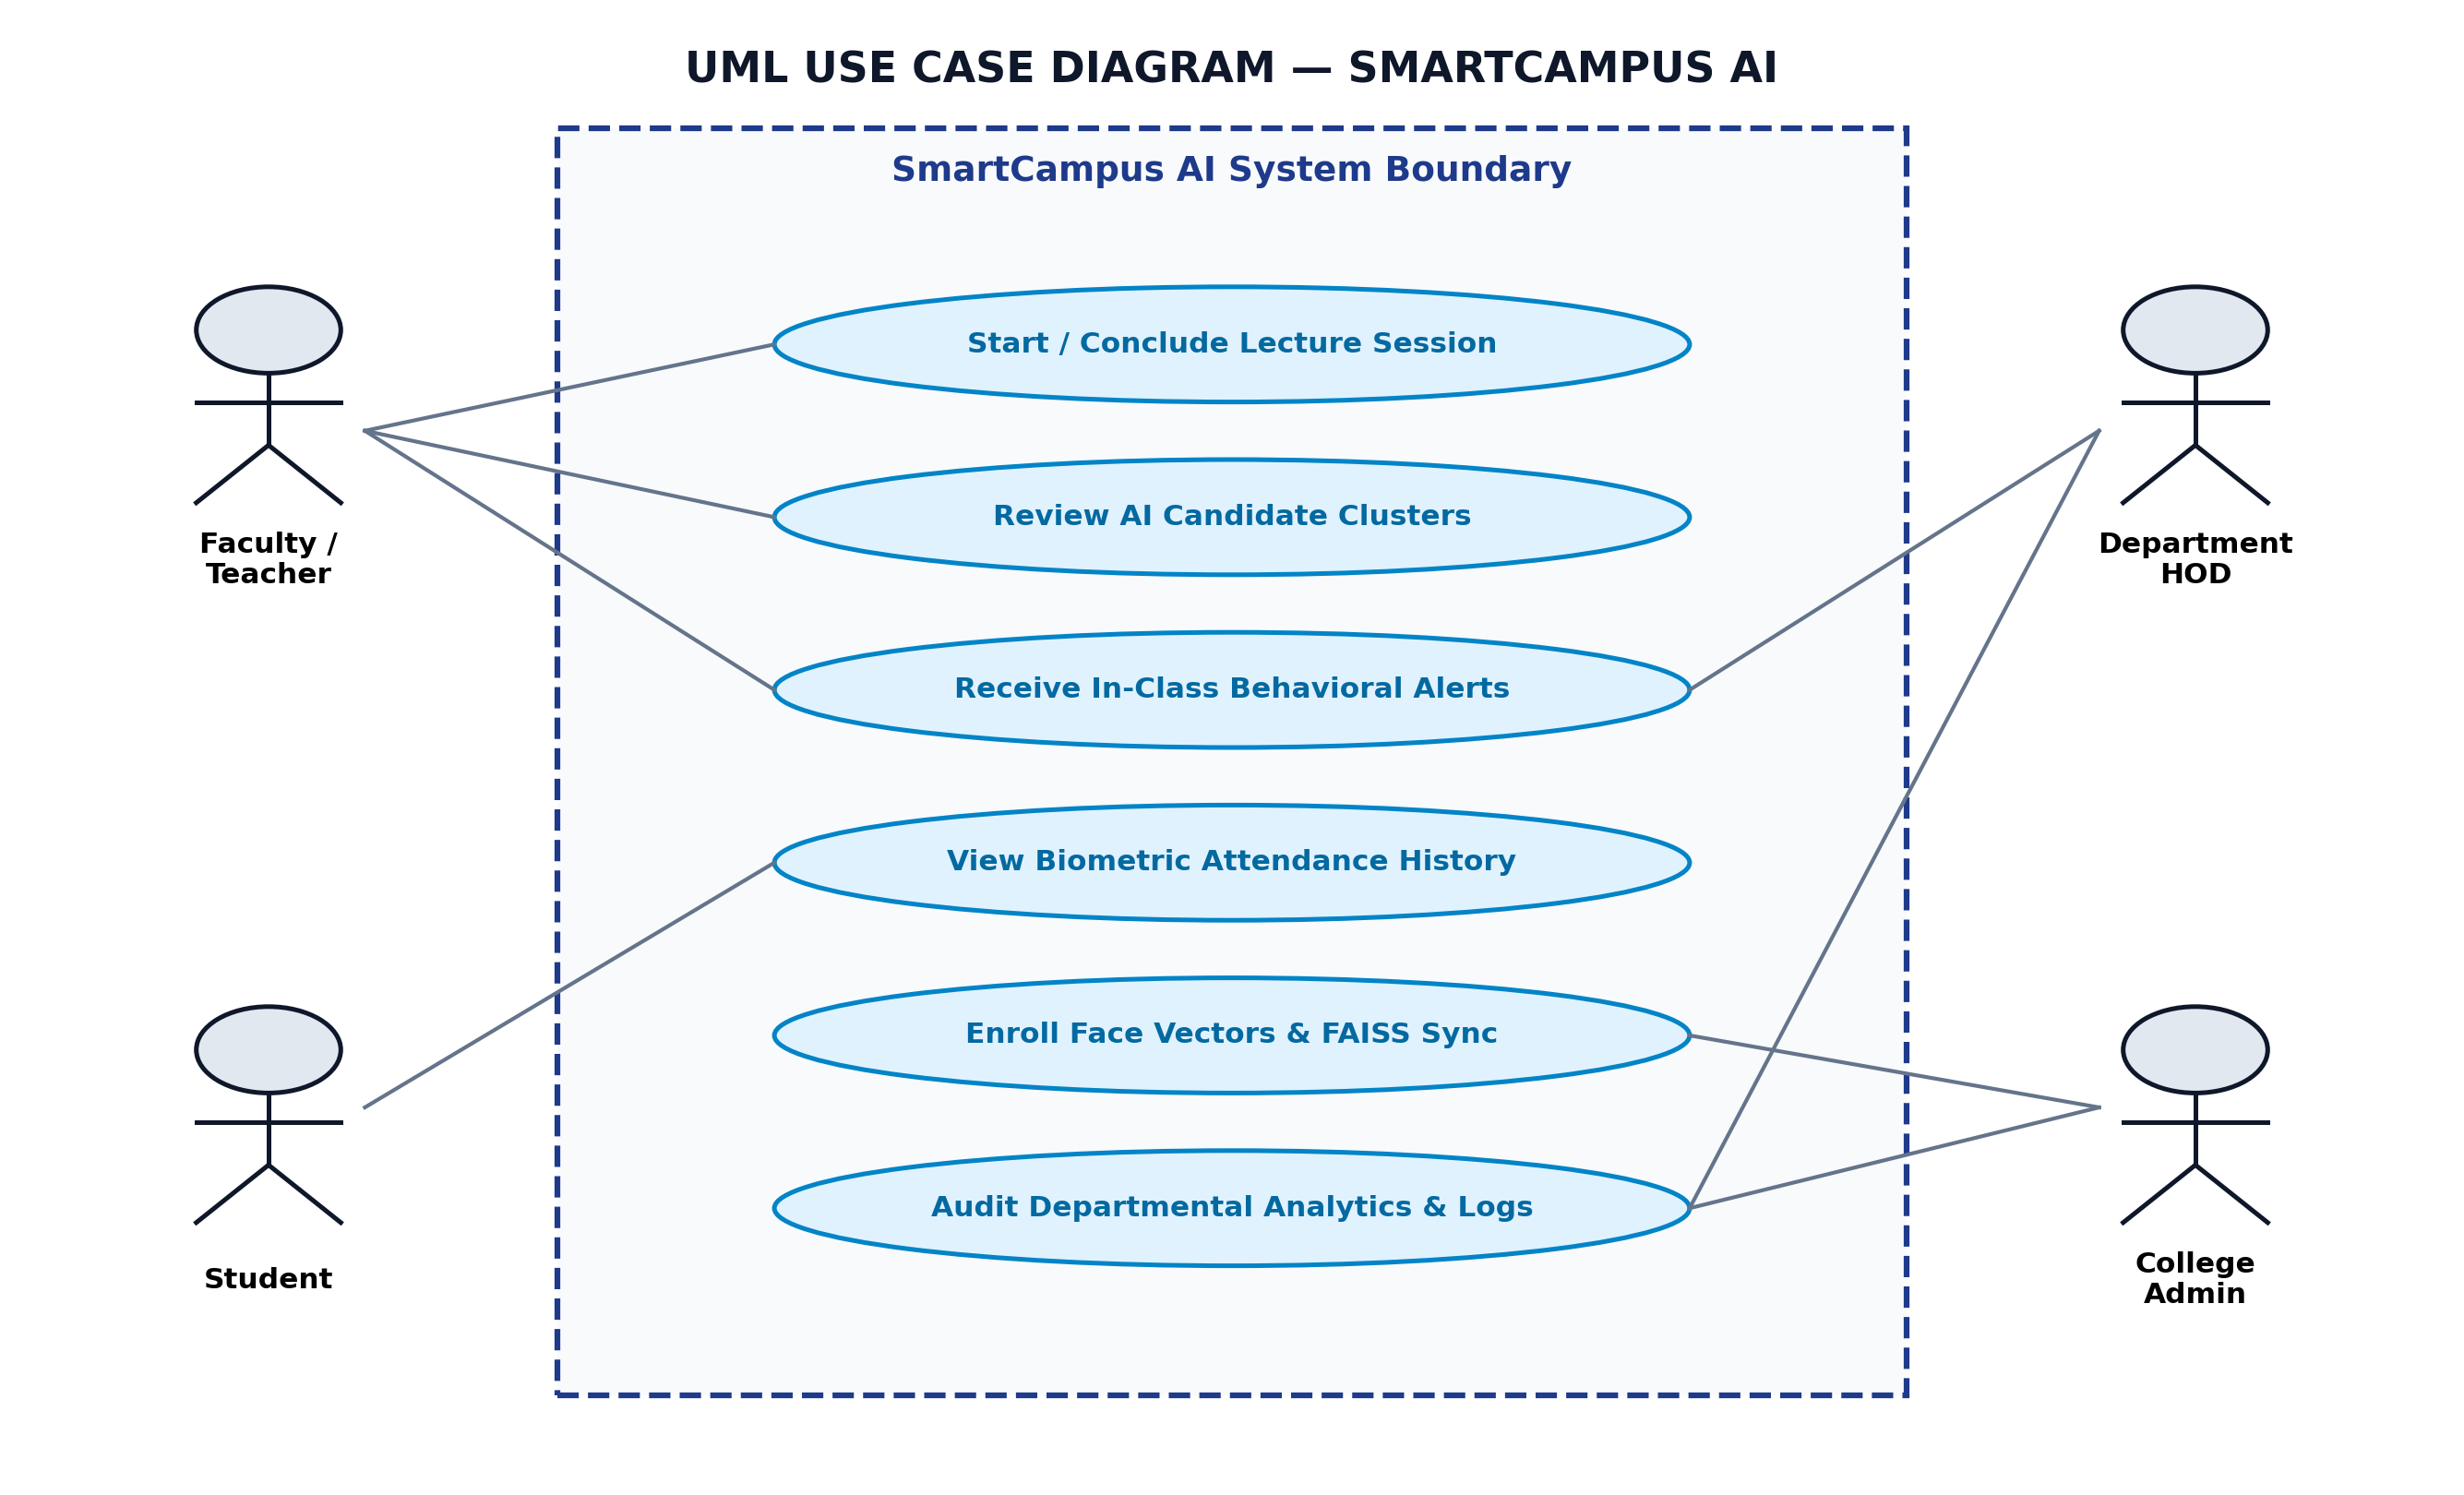
\includegraphics[width=0.88\textwidth]{assets/fig_usecase.png}
    \caption{Use Case Diagram of SmartCampus AI}
    \label{fig:usecase_model}
\end{figure}

\vspace{0.2in}
\begin{flushleft}
{\fontsize{14pt}{18pt}\selectfont \textbf{5.7 SEQUENCE DIAGRAM}}\\[2mm]
\end{flushleft}
\addcontentsline{toc}{subsection}{\numberline{5.7}Sequence Diagram}

\noindent Figure 5.4 presents the UML Sequence Diagram illustrating the chronological message and data exchanges between the Faculty User, NestJS Gateway, PostgreSQL Database, Python AI Engine, and FAISS Vector Database during an active lecture monitoring session.

\begin{figure}[h]
    \centering
    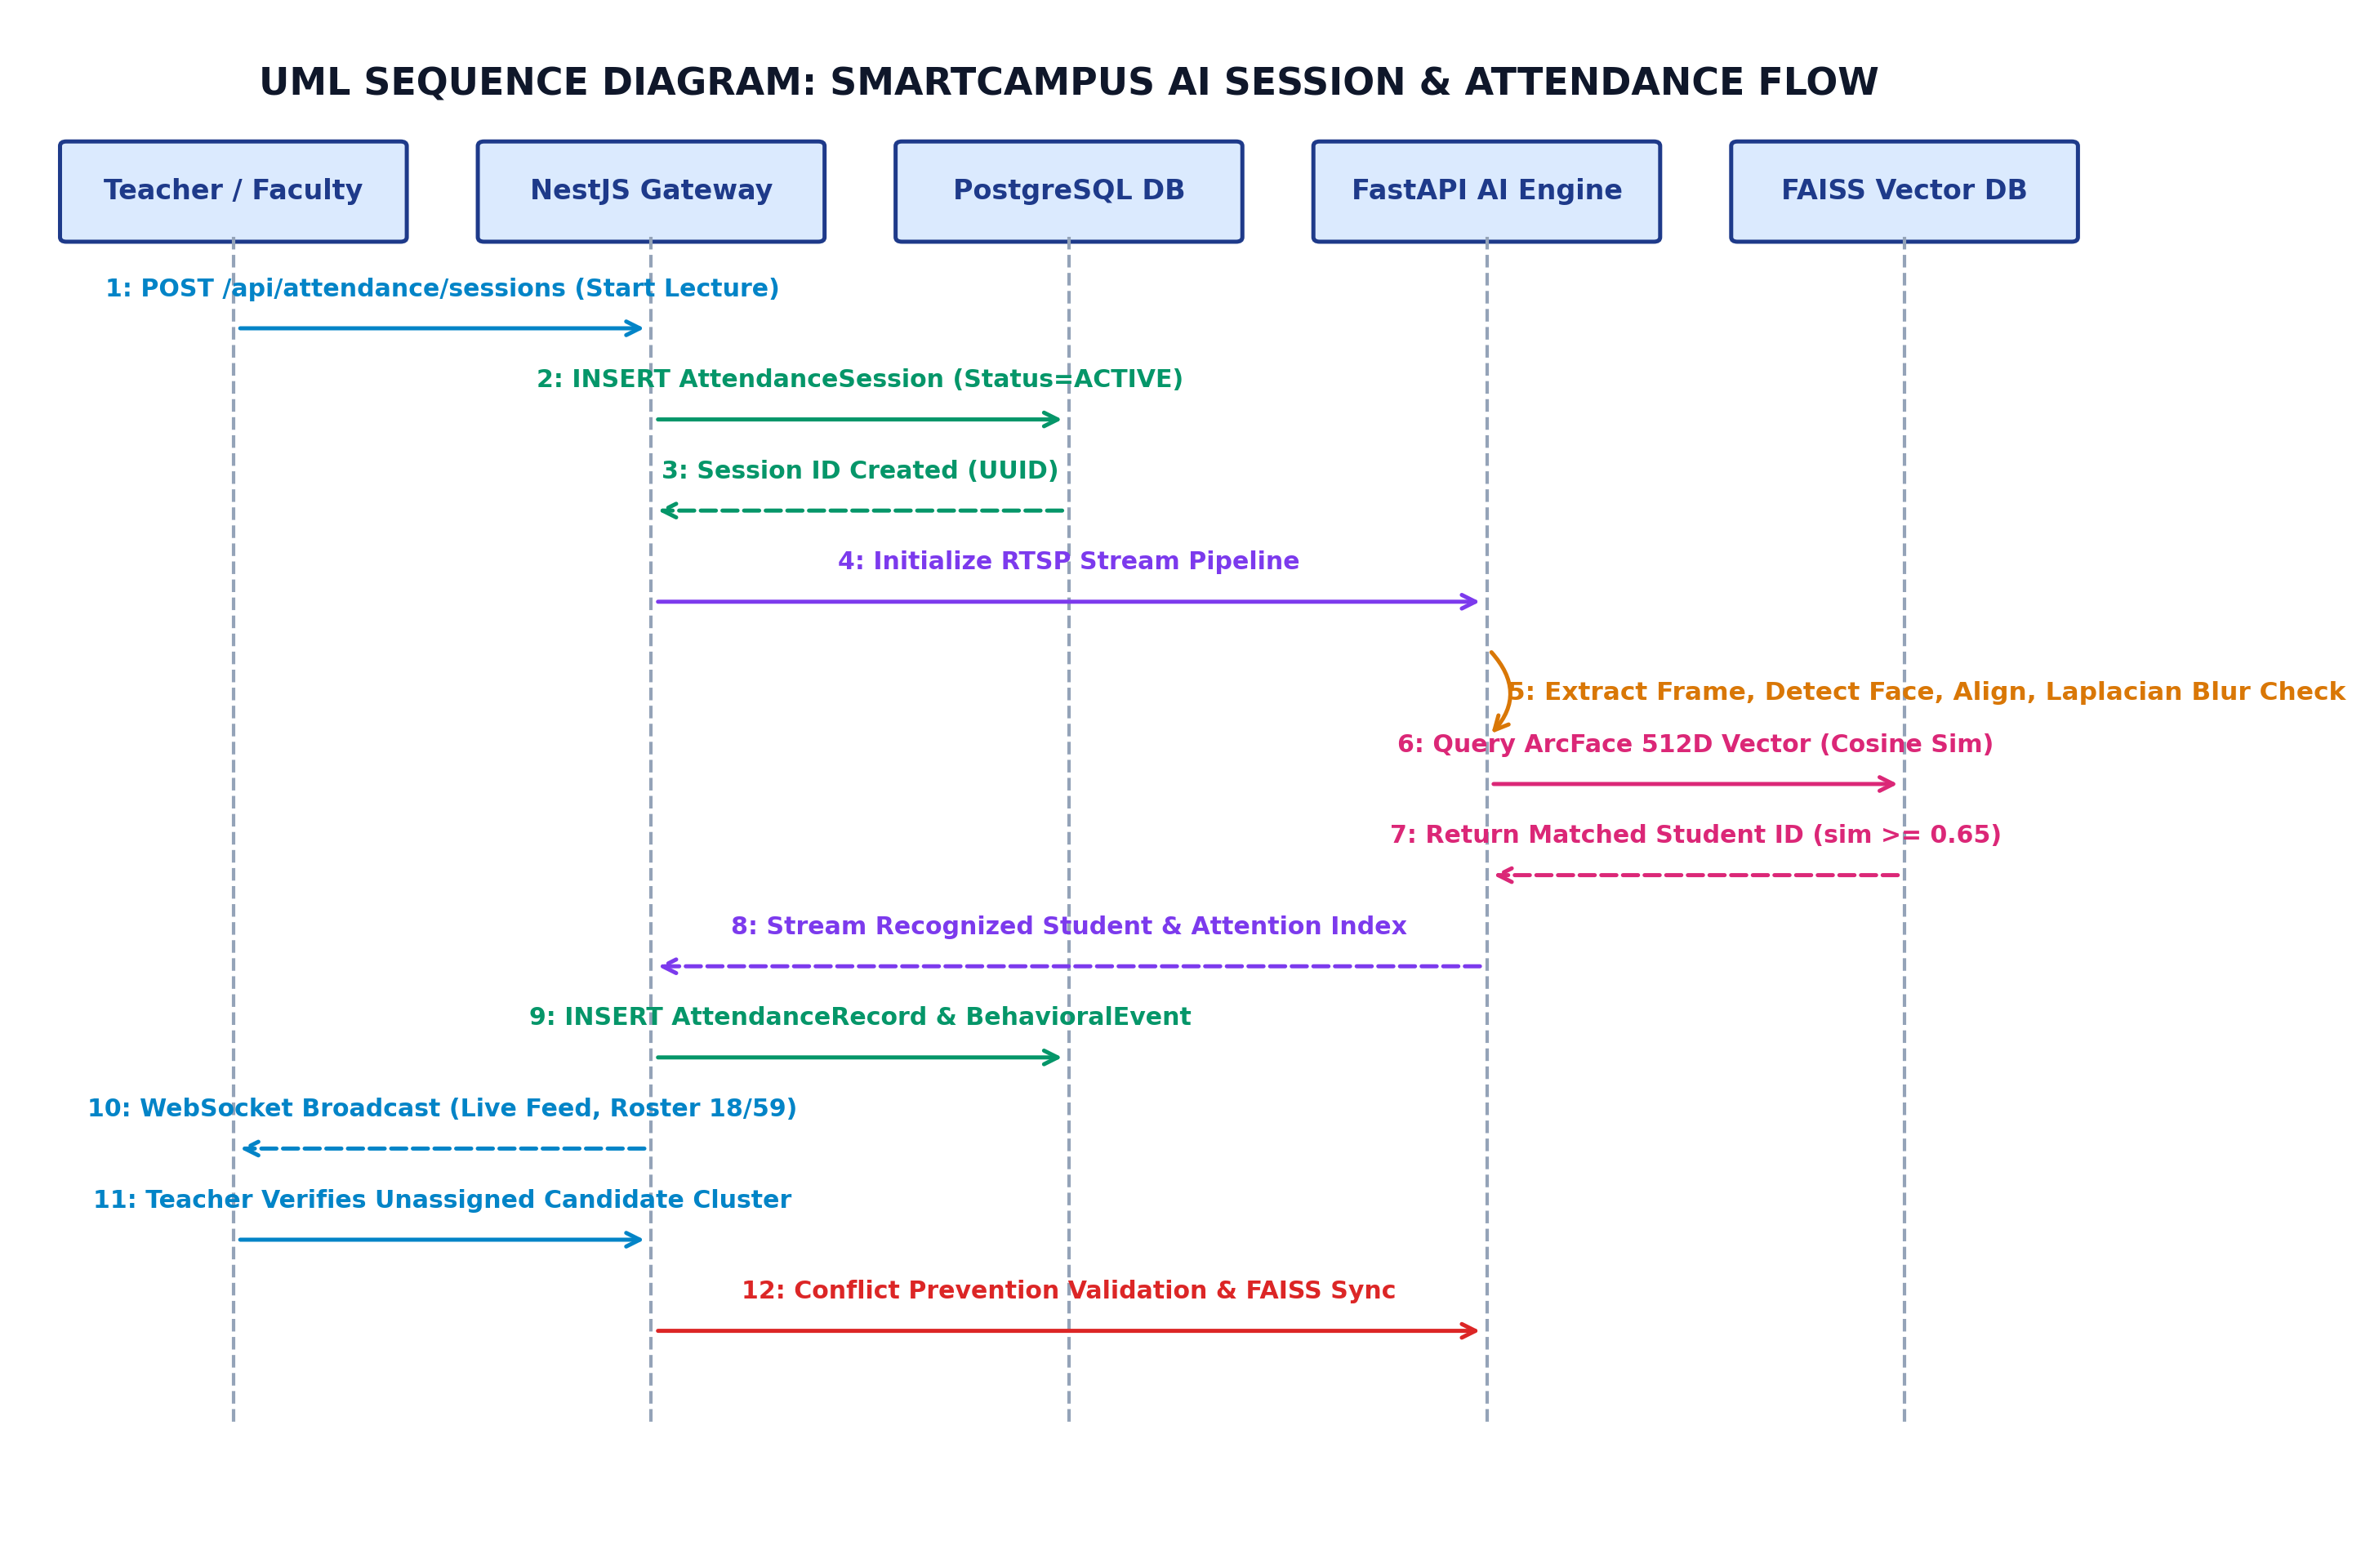
\includegraphics[width=0.92\textwidth]{assets/fig_sequence.png}
    \caption{Sequence Diagram of SmartCampus AI}
    \label{fig:seq_model}
\end{figure}

\noindent As shown in Figure 5.4, the teacher initiates the lecture session via `POST /api/attendance/sessions`. The gateway creates an active session record in PostgreSQL and triggers the AI video pipeline. The vision engine ingests RTSP frames, executes SCRFD face detection, validates Laplacian sharpness, extracts 512D ArcFace embeddings, and queries FAISS. Verified student IDs are committed to PostgreSQL and broadcast via WebSockets to connected dashboards.
\newpage
